\clearpage
% \setcounter{page}{1}
% Reset section numbering to A, B, C...
% \renewcommand{\thesection}{\Alph{section}}  % Use alphabetic section numbering (A, B, C, ...)
% \setcounter{section}{0}  % Reset section counter
\onecolumn


% \maketitlesupplementary
% \onecolumn
% \begin{center}
%     \Large 
%     \textbf{Medverse: A Universal Model for Full-Resolution 3D Medical Image Segmentation, Transformation and Enhancement}\\
%     \vspace{0.5em}Supplementary Material \\
%     \vspace{1.0em}
% \end{center}

\begin{figure*}[t]
\centering
\Large 
\textbf{Medverse: A Universal Model for Full-Resolution 3D Medical Image Segmentation, Transformation and Enhancement} \\[0.5em]
Supplementary Material \\[1.0em]
\end{figure*}

\section{Related Work}
\label{sec:related}

\subsection{Domain Diversity in Medical Imaging}

Medical imaging data exhibits high variability across multiple axes, including anatomical regions, imaging modalities (e.g., CT, MRI, PET, Ultrasound), acquisition settings, and institutions~\cite{bell2022harmonization, zhang2020generalizing}. This diversity poses significant challenges for conventional models, which are typically trained on narrow, task-specific datasets, resulting in poor generalization to unseen domains. Researchers have explored domain adaptation approaches~\cite{wang2023fvp, hu2024chebyshev}, which involve fine-tuning models on the target domain. However, this requirement limits their scalability and makes wide deployment in clinical settings difficult. Domain generalization methods have also been proposed to overcome this limitation without requiring target-domain fine-tuning. These methods either expand the training distribution via predesigned strategies~\cite{zhang2020generalizing, ouyang2022causality}, or attempt to learn domain-invariant features~\cite{hu2022domain, ilse2020diva}. Nevertheless, their effectiveness in overcoming domain shift remains limited and their performance gains are often unstable. Recently, training universal models on large-scale and diverse datasets has emerged as a promising solution to address domain shift in medical imaging~\cite{butoi2023universeg, ma2024segment, hu2025building}. These models demonstrate strong generalization capabilities across institutions, imaging modalities, and even tasks, making them ideal choices for deployment in clinical centers.


\subsection{In-Context Learning in Medical Imaging}

In-Context Learning (ICL) has emerged as a powerful paradigm for performing multiple tasks by conditioning inference on a small set of examples, known as contexts, without modifying model parameters. ICL was first introduced in the field of natural language processing~\cite{brown2020language}, and has been shown to generalize effectively to out-of-distribution data~\cite{reddy2023mechanistic, chan2022data}. As a result, ICL is increasingly viewed as a promising approach for overcoming domain shift in computer vision. Models such as SegGPT~\cite{wang2023seggpt} and Painter~\cite{wang2023images} have demonstrated the potential of ICL across a wide range of vision tasks. In the medical imaging domain, UniverSeg and Neuralizer—based on convolutional and multi-branch architectures—have validated the effectiveness of ICL for 2D segmentation tasks and 2D neuroimaging tasks, respectively. ICL-SAM~\cite{hu2024icl} combines the ICL model with SAM, further improving the performance of ICL models on 2D medical imaging segmentation tasks. Building on these works, Neuroverse3D further extended ICL to the 3D setting while reducing the memory burden of ICL modules, demonstrating promising results in 3D neuroimaging applications. However, Neuroverse3D remains limited to neuroimaging and struggles to handle high-resolution 3D medical images, which constrains its applicability in broader clinical scenarios. Building ICL frameworks that can apply to diverse medical scenarios and high-resolution 3D images remains an open challenge.



\subsection{Universal Models in Medical Imaging}
A growing number of universal models have been developed in medical imaging, particularly for segmentation tasks~\cite{ma2024segment, wong2024scribbleprompt,liu2023clip, ye2023cardiacseg}. Prompt-based universal models include those that utilize point and bounding box inputs, such as SAM~\cite{kirillov2023segment} and MedSAM~\cite{ma2024segment}, as well as ScribblePrompt~\cite{wong2024scribbleprompt}, which incorporates scribble annotations, and nnInteractive, which extends these methods to 3D. These approaches have shown promising results. However, a key difference is that such models require manual input for each image, such as interactive annotations, whereas ICL models require no manual intervention once context examples are provided. These two types of models can be applied in different scenarios—or even combined, as explored in~\cite{hu2024icl}. Moreover, since ICL models take image-label pairs as input, they can be naturally extended to support a wider range of tasks, including image transformation and enhancement. Another line of work has explored natural language prompts to instruct models, such as CLIP-based frameworks adapted to the medical domain~\cite{liu2023clip, liu2024universal}. While these models exhibit strong generalization capabilities, their reliance on textual input makes it difficult for them to generalize beyond pre-defined targets or tasks seen during training.

\clearpage
\section{Autoregressive Inference Pipeline of Medverse}
\begin{algorithm}[h]
\caption{Autoregressive Inference Pipeline of Medverse}
\label{alg:medverse_inference}
\begin{algorithmic}[1]  % 1 = 每行显示行号
\Require Target volume $\bm{x}\in\mathbb{R}^{H\times W\times D}$; 
        semantic context $S\in\mathbb{R}^{L\times 2 \times H\times W\times D}$ 
        (where $L$ is the context size and the second dimension indexes the image–label pairs); 
        patch size $I$; 
        prediction network $F(\cdot)$
\Ensure  Final prediction $\hat{\bm{y}}\in\mathbb{R}^{H\times W\times D}$
%
\State $T \gets \bigl\lceil\log_{2}\bigl(\frac{\max\{H,W,D\}}{I}\bigr)\bigr\rceil + 1$
       \Comment{number of autoregressive steps}
\State $\mathcal{A}^{(0)} \gets \varnothing$ \Comment{empty autoregressive context}
%
\For{$t = 1$ \textbf{to} $T$}                       \Comment{coarse $\rightarrow$ fine}
    \State $H^{(t)}\!\gets\!\lceil H / 2^{\,T-t}\rceil,\;
           W^{(t)}\!\gets\!\lceil W / 2^{\,T-t}\rceil,\;
           D^{(t)}\!\gets\!\lceil D / 2^{\,T-t}\rceil$
    \State Resize $\bm{x}$ and $S$ to $\bigl(H^{(t)},W^{(t)},D^{(t)}\bigr)$
    %
    \If{$t == 1$}          \Comment{global low-resolution prediction}
        \State $\hat{\bm{y}}^{(1)} \gets
               F\bigl(\bm{x}^{(1)},\, S^{(1)},\, \mathcal{A}^{(0)}\bigr)$
    \Else                   \Comment{patch-wise refinement}
        \State Divide $\bm{x}^{(t)}$ into (possibly overlapping) patches
               $\{\bm{x}^{(t)}_i\}$ of size $I^3$
        \ForAll{patch index $i$}
            \State Crop aligned semantic context $S^{(t)}_i$
            \State Extract corresponding region
                   $\mathcal{A}^{(t-1)}_i$ from $\mathcal{A}^{(t-1)}$
                   and upsample to $I^3$
            \State $\hat{\bm{y}}^{(t)}_i \gets
                   F\bigl(\bm{x}^{(t)}_i,\,
                          S^{(t)}_i,\,
                          \mathcal{A}^{(t-1)}_i\bigr)$
        \EndFor
        \State Aggregate $\{\hat{\bm{y}}^{(t)}_i\}$
               to obtain $\hat{\bm{y}}^{(t)}$
    \EndIf
    \State $\mathcal{A}^{(t)} \gets \bigl(\bm{x}^{(t)},\, \hat{\bm{y}}^{(t)}\bigr)$
           \Comment{update AR context}
\EndFor
%
\Return $\hat{\bm{y}}^{(T)}$
\end{algorithmic}
\end{algorithm}



\section{Experiments Setting}
\label{sec:data_sup}
% 数据表格

\begin{table*}[h!]
    \centering
    \renewcommand{\arraystretch}{1.1}
    \setlength{\tabcolsep}{4pt}
    \resizebox{0.85\textwidth}{!}{
    \begin{tabular}{cccccc>{\centering\arraybackslash}p{3cm}}
        \toprule
        \textbf{Type for use} & \textbf{Dataset}& \textbf{Organ} & \textbf{Task} & \textbf{\# Scans} & \textbf{\# Masks} & \textbf{Modality} \\
        \midrule
        % \textbf{Training Set} & & & & & \\
        \multirow{17}{*}{\begin{tabular}[x]{@{}c@{}}Training and \\Validation Set\end{tabular}} 
        & TopCow~\cite{yang2023benchmarking} & Brain & Seg., Enh. & 90 & 90 & MRA \\
        & CAS2023~\cite{CAS2023} & Brain & Seg., Enh.  & 100 & 100 & MRA \\
        & ISLES2022~\cite{hernandez2022isles} & Brain & Enh., Tran.  & 750 & 0 & \renewcommand{\arraystretch}{0.8}\begin{tabular}[x]{@{}c@{}}DWI, ADC,\\FLAIR\end{tabular}\\
        & ATLAS~\cite{liew2022large} & Brain & Seg., Enh. & 655 & 655 & T1w \\
        & IXI~\cite{IXI} & Brain & Enh., Tran.  & 2268 & 0 &   \renewcommand{\arraystretch}{0.8}\begin{tabular}[x]{@{}c@{}}T1, T2,\\MRA, PD\end{tabular}\\
        & ICH Unlabeled~\cite{flanders2020construction} & Brain & Enh.  & 2000 & 0 & CT \\
        & ADHD~\cite{ADHD} & Brain & Seg., Enh., Tran.  & 950 & 200 & T1 \\
        & ADNI~\cite{jack2008alzheimer} & Brain & Seg., Enh., Tran. & 9923 & 200 & T1 \\
        & CMI~\cite{alexander2017open} & Brain & Seg., Enh., Tran.  & 5146 & 200 & T1 \\
        & GSP~\cite{holmes2015brain} & Brain & Seg., Enh., Tran.  & 2616 & 200 & T1 \\
        & HAB~\cite{gera2023characterizing} & Brain & Seg., Enh., Tran.  & 460 & 460 & T1 \\
        & NIMH~\cite{nugent2022nimh} & Brain & Seg., Enh., Tran.  & 248 & 248 & T1 \\
        & OASIS~\cite{marcus2007open} & Brain & Seg., Enh., Tran.  & 3916 & 828 & T1 \\
        & UKBiobank~\cite{sudlow2015uk} & Brain & Seg., Enh.  & 4000 & 2000 & T1, T2 \\
        & BraTS~\cite{menze2014multimodal} & Brain & Seg., Enh., Tran.  & 5004 & 1251 & \renewcommand{\arraystretch}{0.8}\begin{tabular}[x]{@{}c@{}}FLAIR, T1,\\T1CE, T2\end{tabular} \\
        & WMH~\cite{kuijf2019standardized} & Brain & Enh., Tran. & 120 & 0 & T1, FLAIR \\
        & PROMISE12~\cite{litjens2014evaluation} & Prostate & Seg., Enh. & 50 & 50 & T2 \\
        & CAS~\cite{zeng2023imagecas} & Cardiac & Seg., Enh. & 190 & 190 & CTA \\
        & AMOS22~\cite{ji2022amos} & Abdomen & Seg., Enh. & 360 & 360 & CT \\
        & RAOS~\cite{luo2024rethinking} & Abdomen & Seg., Enh. & 317 & 317 & CT \\
        & TotalSeg~\cite{wasserthal2023totalsegmentator} & Abdomen & Seg., Enh. & 87 & 87 & CT \\
        & MSD~\cite{antonelli2022medical} & Lung, Cardiac & Seg., Enh. & 83 & 83 & CT \\
        

        
        \midrule
        % \textbf{Held-out Set} & & & & & \\
        \multirow{5}{*}{Held-out Set} 
        & PPMI~\cite{marek2011parkinson} & Brain & Seg., Enh., Tran.  & 220 & 220 & T1 \\
        & FLARE22~\cite{ma2024unleashing} & Abdomen & Seg., Enh.  & 50 & 50 & CT \\
        & Nasal~\cite{zhang2024nasalseg} & Nasal & Seg., Enh.  & 130 & 130 & CT \\
        & Mice~\cite{rosenhain2018preclinical} & Body & Seg., Enh.  & 40 & 40 & CT \\
        & ADNI\cite{jack2008alzheimer} & Brain & Seg., Enh.  & 589 & 589 & PET \\
        % & IXI~\cite{IXI} & Brain & Tran.  & 1134 & 0 &  PD$\rightarrow$T2\\
        \midrule

        & \textbf{Total} & \renewcommand{\arraystretch}{0.8}\begin{tabular}[x]{@{}c@{}}Brain, Lung,\\ Abdomen, Cardiac\\ Prostate, Nasal\end{tabular} & Seg., Enh., Tran. & 40362 & 8548 & \renewcommand{\arraystretch}{0.8}\begin{tabular}[x]{@{}c@{}}T1, T2, FLAIR,\\MRA, DWI, ADC,\\ PD, CT, PET\end{tabular} \\
        
        \bottomrule
    \end{tabular}}
    \caption{Summary of datasets. Segmentation, enhancement, and transformation tasks are denoted as Seg., Enh., and Tran., respectively. The PET modality data from the ADNI dataset was not included in training.}

    \label{tab:dataset_summary}
\end{table*}


\begin{figure}[h]
\centering
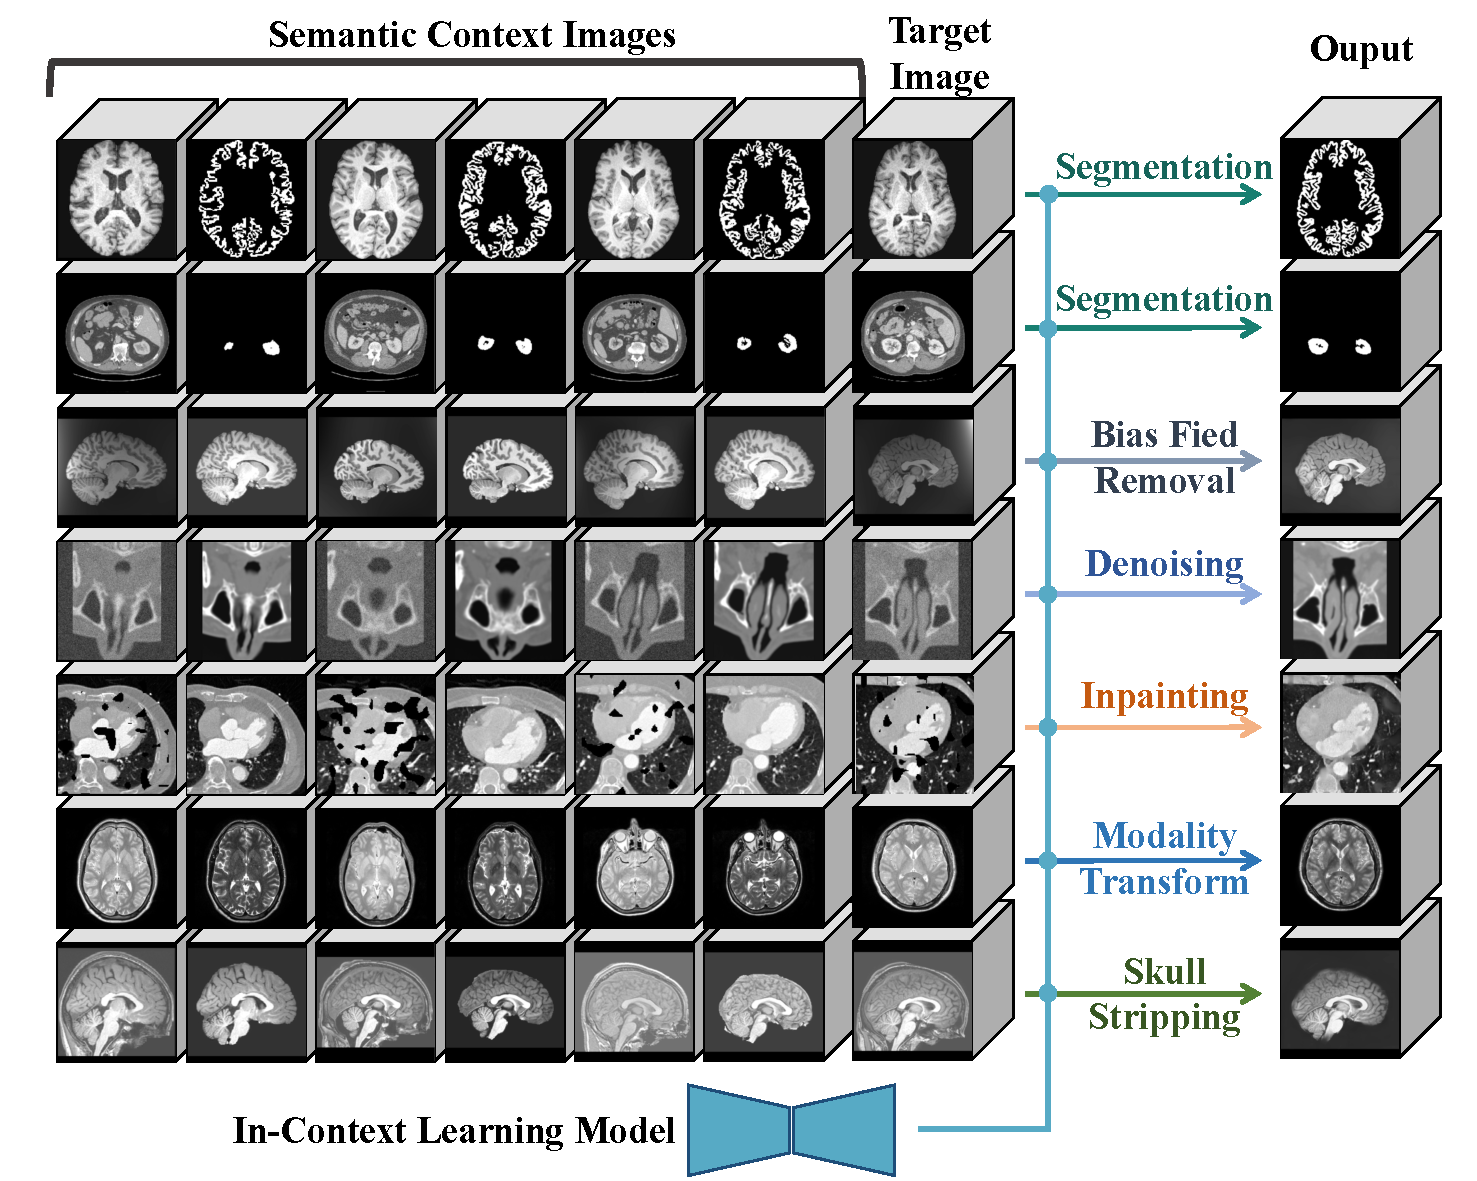
\includegraphics[width=0.45\textwidth]{intro.pdf}
\caption{An overview of tasks executable by the model.}
\label{fig:intro}
\end{figure}

\subsection{Data Sampling}
\label{sec:data_sup_}

During training, tasks are selected according to a predefined sampling distribution.  
For each selected task, a dataset is randomly chosen with equal probability.  
Given a context size of $L$, we randomly sample $L+1$ image–label pairs from the training split of the selected dataset.  
One of these samples is alternately assigned as the target image and corresponding ground truth, while the remaining $L$ samples constitute the context set, following the same protocol as described in~\cite{hu2025building}.  
The sampling distribution over tasks is summarized in Table~\ref{tab:task_sampled_weight}.

\begin{table}
\centering
\renewcommand{\arraystretch}{1} % Adjust row height
\resizebox{0.47\textwidth}{!}{
    \begin{tabular}{ccc}
    \toprule
    \textbf{Task} & \textbf{Sampled Rate} & \textbf{Weight} \\
    \midrule
    Segmentation & 3 & 50 \\
    Bias Remove & 2 & 1 \\
    Gaussian Noise Remove & 2 & 1 \\
    Salt \& Pepper Noise Remove & 2 & 1 \\
    Inpainting & 2 & 1 \\
    Skull Stripping & 1 & 1 \\
    Modality Transform & 1 & 1 \\
    \bottomrule
    \end{tabular}
    }
    \caption{Sampling rate and weight for each task during training.}
\label{tab:task_sampled_weight}
\end{table}

\subsection{Task Construction}
\label{sec:tasks_sup}

\vspace{0.4em}\noindent\textbf{Segmentation:} Our model performs binary segmentation. For multi-class segmentation datasets, each class is treated as the foreground in turn, while all other classes are merged into the background.  For prediction, binary masks were produced by thresholding the model outputs at 0.5. 

\vspace{0.4em}\noindent\textbf{Skull Stripping:} The objective is to remove the skull region from brain images~\cite{hoopes2022synthstrip}. Ground-truth skull-stripping masks are generated using FreeSurfer~\cite{fischl2012freesurfer} from T1-weighted brain images. For this task, we performed evaluation on a held-out subset of the PPMI dataset.

\vspace{0.4em}\noindent\textbf{Modality Transformation:} This task converts images from one modality to another, where the input and output volumes are spatially registered. For this task, we evaluated on the PD$\rightarrow$T2 modality transformation task from the IXI dataset, as the modalities in this dataset are well spatially aligned, making it suitable for evaluation. Moreover, the PD$\rightarrow$T2 task was excluded from the training tasks.


\vspace{0.4em}\noindent\textbf{Bias-Field Correction:} The goal is to correct intensity inhomogeneities in MRI scans~\cite{goldfryd2021deep}. Three-dimensional bias fields are synthesized using Legendre polynomials with randomly sampled coefficients. For all enhancement tasks, we perform evaluation on five held-out sets and report the average results.

\vspace{0.4em}\noindent\textbf{Gaussian Noise Removal:} This task is synthesized by adding zero-mean Gaussian noise with a standard deviation uniformly sampled from the range 0.15 to 0.25.

\vspace{0.4em}\noindent\textbf{Salt-and-Pepper Noise Removal:} This task is synthesized by introducing salt noise (intensity 1) and pepper noise (intensity 0) independently with a probability of 0.04.

\vspace{0.4em}\noindent\textbf{Inpainting:} The objective is to reconstruct missing or occluded regions in the input image~\cite{liu2021symmetric}. This task is synthesized using binary masks generated from random three-dimensional Perlin noise to occlude regions of the input.



\subsection{Image and Task Augmentation}
\label{sec:aug}

Image and task augmentation are critical for training in-context learning models and are applied after data sampling.  
For image augmentation, we applied the following transformations: random affine transformations (probability 0.05), elastic deformations (0.05), flipping (0.05), and rotations (0.05).  
To further increase image diversity, we introduced random intensity shifts (0.2), intensity scaling (0.2), Gaussian noise (0.1), and intensity inversion (0.05).

For task augmentation, we employed several strategies, including Sobel filtering, mask inversion, random dilation, random erosion, task overlapping, and foreground randomization, following the procedures described in~\cite{hu2025building}.

\vspace{0.4em}
\noindent\textbf{GIN.}
We also applied a random convolutional network known as GIN~\cite{ouyang2022causality} (0.05), which generates images with randomized contrast.

\vspace{0.4em}
\noindent\textbf{Synthetic Data.}
We incorporated synthetic data following~\cite{butoi2023universeg, hoffmann2021synthmorph}.  
We used randomly sampled binary masks, brain masks, and abdomen masks derived from TotalSegmentator~\cite{wasserthal2023totalsegmentator} to generate synthetic images.  
This process resulted in 150 synthetic segmentation datasets with varying contrast properties, each containing 100 three-dimensional image samples.


\subsection{Training}
During training, we adopt a teacher forcing approach, where the autoregressive context is replaced with ground-truth image-label pairs downsampled by a factor of 2. To prevent the model from over-relying on the autoregressive context—since it may be imperfect during actual inference—we introduce noise by using a larger downsampling factor. Specifically, instead of consistently using a factor of 2, we randomly sample the downsampling factor from the set \{2, 3, 4\} for the ground truth.

Medverse was trained on 2 NVIDIA A100 80GB GPUs with a batch size of 1 per GPU, using the ADAM optimizer.  
Training was conducted for 240K steps with an initial learning rate of $3\times 10^{-5}$.  
Validation loss was evaluated every 2.4K steps, and the learning rate was reduced by half if no improvement was observed over 20 consecutive evaluations.  
To improve training efficiency, the context size and mini-context size were fixed at three for the first 200K steps, requiring the model to process only a single mini-context.  
For the remaining 40K steps, the context size was uniformly sampled between 1 and 8.  
Training was completed in approximately 8 days, and the model with the lowest validation loss was selected for evaluation.
All task-specific models were trained on a single GPU for 36{,}000 steps due to the significantly smaller training sets and faster convergence.

\subsection{Evaluation}
We evaluate model performance using two standard metrics in medical image analysis: Dice coefficient and Peak Signal-to-Noise Ratio (PSNR). Dice is used for segmentation tasks and measures the spatial overlap between the predicted and ground truth masks. It is particularly suitable for medical segmentation due to its robustness to class imbalance. PSNR is used for image transformation and enhancement tasks. It quantifies the pixel-level similarity between the predicted and reference images, reflecting the fidelity of the output. Together, these metrics provide a comprehensive evaluation of both structural accuracy and image quality. Each task and setting was repeated 8 times with randomly sampled context sets.  
The average and standard deviation across runs were reported to ensure robust performance estimation.


\section{Additional Experiments}
% \vspace{0.4em}
% \noindent\textbf{Comparison of Context Cropping Strategies.}
% Figure~\ref{fig:crop} illustrates the impact of different cropping strategies on model performance during sliding-window processing. In the position-aligned cropping strategy, the spatial location of the cropped region in the context image is aligned with that in the target image. In contrast, the random foreground cropping strategy randomly selects regions from the context that contain foreground structures, thereby providing task-relevant guidance and avoiding the inclusion of entirely background regions. As shown in the figure, when the NSA-ICL framework is not used, the model is highly sensitive to the cropping strategy. Random foreground cropping leads to a significant drop in performance, indicating that the model remains sensitive to spatial misalignment. However, when the NSA-ICL framework is incorporated, the performance of random foreground cropping improves substantially, and the gap between the two strategies narrows. This is attributed to the global semantic information provided by the autoregressive branch, which enhances task guidance. In other words, the NSA-ICL framework improves the model's robustness to different context cropping strategies.


% \begin{figure}
% \centering
% \includegraphics[width=0.47\textwidth]{random_crop.pdf}
% \caption{Model comparison of context random crop and aligning crop.}
% \label{fig:crop}
% \end{figure}


% \vspace{0.4em}
% \noindent\textbf{Impact of Context Construction Strategies.}
% Figure~\ref{fig:context_con} illustrates the effects of different context construction strategies during sliding-window inference. Selecting an appropriate strategy for cropping context patches is critical. In this study, we investigate several approaches. \emph{Aligned cropping} extracts context patches from spatially aligned positions with the target image. \emph{Random cropping} samples regions from the context that contain foreground structures. \emph{Whole image} includes a downsampled version of the entire volume as part of the context set. These three methods do not incorporate autoregressive guidance. Our NSA-ICL framework can be viewed as introducing an additional autoregressive context, forming a new context construction strategy. As shown in the figure, \emph{random cropping} leads to a substantial performance drop compared to \emph{aligned cropping}, indicating that anatomical alignment across samples plays a key role in effective context-based learning. This also highlights the sensitivity of ICL models to spatial consistency between the target and context. While incorporating the \emph{whole image} as global guidance appears promising, it fails to improve performance and even causes degradation, suggesting that the model struggles to directly extract task-relevant information from coarse-resolution global context. Note that we fine-tune the model for both \emph{random cropping} and \emph{whole image} strategies to ensure consistency between training and inference. Finally, incorporating the autoregressive context via our NSA-ICL framework consistently improves performance across segmentation, transformation, and enhancement tasks, demonstrating the effectiveness of our proposed approach.

% \begin{figure}
% \centering
% 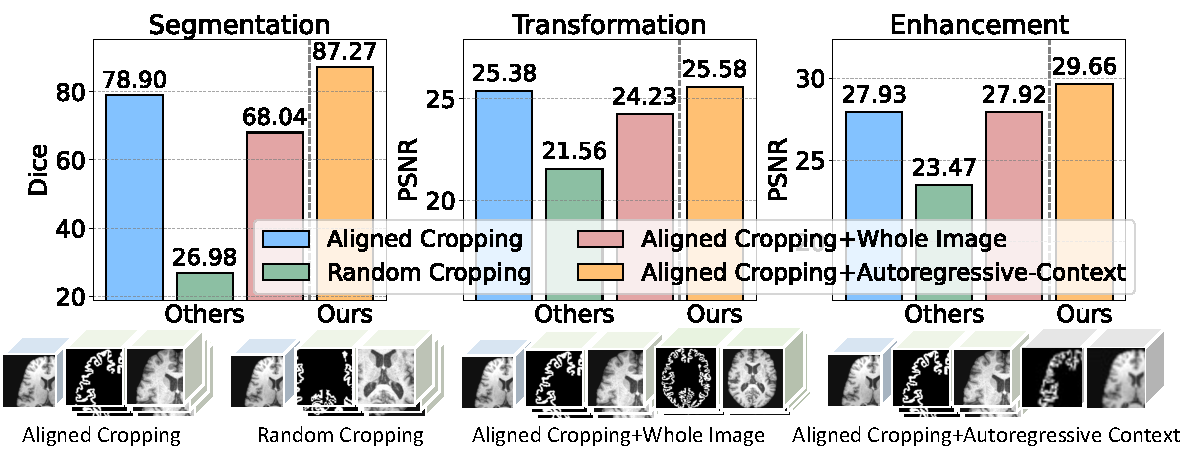
\includegraphics[width=0.47\textwidth]{context_strategy.pdf}
% \caption{Comparison of context construction strategies during sliding-window inference. \emph{Aligned cropping} uses the same spatial positions as the target image. \emph{Random cropping} selects foreground regions randomly. \emph{Whole image} adds downsampled full images as context.}
% \label{fig:context_con}
% \end{figure}

\vspace{0.4em}
\noindent\textbf{Comparison of Context Construction Strategies.}  
Figure~\ref{fig:context_con} shows the impact of various context construction strategies. NA-ICL introduces an additional autoregressive context, forming a novel strategy. We fine-tuned models under corresponding strategies to ensure a fair comparison. Compared to aligned cropping, random cropping significantly reduces performance, indicating that anatomical alignment across samples is crucial for effective context learning. Directly incorporating the whole image as global context does not improve performance and can even degrade it suggesting that it is difficult to leverage coarse-resolution guidance directly across scales. Incorporating autoregressive context consistently improves performance across all kinds of tasks, highlighting the strength of our approach.


\begin{figure}
\centering
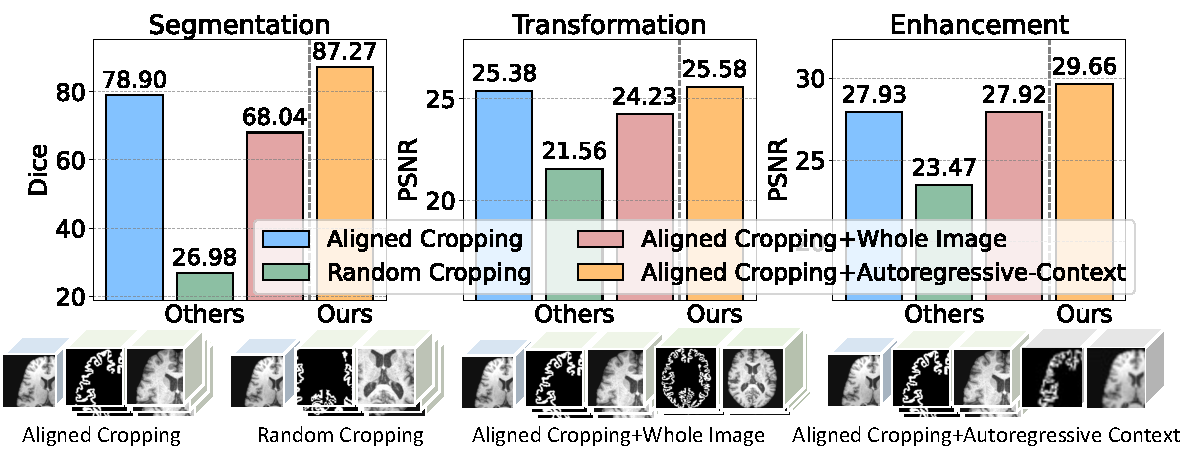
\includegraphics[width=0.7\textwidth]{context_strategy.pdf}
\caption{Comparison of different context construction strategies during sliding-window inference. Aligned Cropping+Autoregressive Context represents our proposed method. Random Cropping selects crops randomly from foreground regions. Whole Image adds downsampled full images as context.}
\label{fig:context_con}
\end{figure}

\vspace{0.4em}
\noindent\textbf{Comparison of the computational resources of BAM.}
Table~\ref{tab:compute} compares the computational cost of the BAM module and standard cross-attention. As shown in the table, BAM achieves a substantial reduction in computation, particularly at Stage 1. This is because the spatial size of the features in Stage 1 is large, leading to millions of tokens if standard cross-attention is used, which results in an extremely high computational cost. In contrast, BAM maintains a fixed number of tokens at \( p^3 \), regardless of spatial size. Overall, BAM consistently maintains lower FLOPs and memory usage, while still enabling long-range interactions. At the bottom of the table, we observe that increasing \( p \) gradually improves performance, reaching an optimal value around \( p = 4 \). This suggests two key insights. First, long-range interactions are essential for providing broader receptive fields, which are particularly beneficial for segmentation tasks. Second, in the medical domain, moderate levels of long-range attention are sufficient, and excessively dense attention may not yield additional gains.


\begin{table*}[htbp]
\centering
\caption{Computation cost, FP32 inference time on A100, and memory consumption during inference of the BAM module across different 3D U-Net stages. The cross-attention refers to standard attention without spatial sparsity. When BAM is configured with \( p = 1 \), the module is equivalent to direct concatenation and thus introduces no additional computation. The bottom of the table compares model performance with different values of \( p \). Due to the prohibitively high computational cost of standard cross-attention, its performance could not be reported. "Total" refers to the combined cost of fusion modules in both the encoder and decoder for 1 context pair.}
\label{tab:compute}
\setlength{\tabcolsep}{6pt}
\begin{tabular}{l l r r r r r}
\toprule
\begin{tabular}[c]{@{}l@{}}Stage\\  (Feature Size) \end{tabular} &
Metric & 
\begin{tabular}[c]{@{}l@{}}BAM\\  $p=1$ \end{tabular}    &
\begin{tabular}[c]{@{}l@{}}BAM\\  $p=2$ \end{tabular}    &
\begin{tabular}[c]{@{}l@{}}BAM\\  $p=4$ \end{tabular}    &
\begin{tabular}[c]{@{}l@{}}BAM\\  $p=8$ \end{tabular}    &
Cross-Attention \\
\midrule
\multirow{4}{*}{\begin{tabular}[c]{@{}l@{}}Stage 1\\ 32$\times$128$\times$128$\times$128\end{tabular}}
& GFLOPs & --	& $6.72\times10^{-2}$&$6.85\times10^{-2}$& $1.39\times10^{-1}$& $1.16\times10^{6}$ \\
& Time (s)  &--	& $3.44\times10^{-6}$ & $3.51\times10^{-6}$ & $7.10\times10^{-6}$ & $5.95\times10^{1}$\\
& Memory (GB) & --	& $1.16\times10^{-5}$  & $3.38\times10^{-5}$ & $2.70\times10^{-4}$ & 1.10 \\
& \# Token & $1$ & $2^3$ & $4^3$ & $8^3$ & $128^3$ \\
\midrule
\multirow{4}{*}{\begin{tabular}[c]{@{}l@{}}Stage 2\\ 64$\times$64$\times$64$\times$64\end{tabular}}
& GFLOPs & --	& $1.69\times10^{-2}$ & $1.84\times10^{-2}$ & $9.03\times10^{-2}$ & $1.81\times10^{4}$ \\
& Time (s)   & --	& $8.65\times10^{-7}$ & $9.44\times10^{-7}$  & $4.63\times10^{-6}$ & $9.3\times10^{-1}$\\
& Memory (GB) & --	& $2.11\times10^{-5}$ & $5.02\times10^{-5}$ & $2.83\times10^{-4}$ & $1.4\times10^{-1}$\\
& \# Token & $1$ & $2^3$ & $4^3$ & $8^3$ & $64^3$ \\
\midrule
\multirow{4}{*}{\begin{tabular}[c]{@{}l@{}}Stage 3\\ 128$\times$32$\times$32$\times$32\end{tabular}}
& GFLOPs & -- &	$4.3\times10^{-3}$ & $6.4\times10^{-3}$ & $8.21\times10^{-2}$ & $2.84\times10^{2}$ \\
& Time (s)  &-- &  $2.23\times10^{-7}$ & $3.26\times10^{-7}$  & $4.21\times10^{-6}$ & $1.45\times10^{-2}$\\
& Memory (GB) &-- &  $4\times10^{-5}$ & $8.35\times10^{-5}$ & $4.31\times10^{-4}$ & $2.54\times10^{-2}$ \\
& \# Token & $1$  & $2^3$ & $4^3$ & $8^3$ & $32^3$ \\
\midrule
\multirow{4}{*}{\begin{tabular}[c]{@{}l@{}}Stage 4\\ 256$\times$16$\times$16$\times$16\end{tabular}}
& GFLOPs &-- &  $1.3\times10^{-3}$ & $4.3\times10^{-3}$ & $8.76\times10^{-2}$ & 4.56 \\
& Time (s)  &-- & $6.9\times10^{-8}$ & $2.20\times10^{-7}$  & $4.49\times10^{-6}$  & $2.34\times10^{-4}$ \\
& Memory (GB) &-- & $7.79\times10^{-5}$ & $1.50\times10^{-4}$& $7.27\times10^{-4}$& $5.34\times10^{-3}$ \\
& \# Token & $1$ & $2^3$ & $4^3$ & $8^3$ & $16^3$ \\
\midrule
\multirow{4}{*}{\begin{tabular}[c]{@{}l@{}}Stage 5\\ 512$\times$8$\times$8$\times$8\end{tabular}}
& GFLOPs &-- & $8\times10^{-4}$ & $5.7\times10^{-3}$& $1.04\times10^{-1}$& $1.03\times10^{-1}$\\
& Time (s)  &-- & $4.2\times10^{-8}$ & $2.91\times10^{-7}$  & $5.33\times10^{-6}$ & $5.32\times10^{-6}$ \\
& Memory (GB) & -- & $1.54\times10^{-4}$ & $2.83\times10^{-4}$& $1.32\times10^{-3}$& $1.32\times10^{-3}$ \\
& \# Token & $1$ & $2^3$ & $4^3$ & $8^3$ & $8^3$ \\
\midrule
\multirow{3}{*}{Total}
& GFLOPs & --	& $1.80\times10^{-1}$&$2.01\times10^{-1}$& $9.01\times10^{-1}$& $2.36\times10^{6}$ \\
& Time (s)  &--	& $9.24\times10^{-6}$ & $1.03\times10^{-5}$ & $4.62\times10^{-5}$ & $1.21\times10^{2}$\\
& Memory (GB) & --	& $4.55\times10^{-4}$  & $9.18\times10^{-4}$ & $4.74\times10^{-3}$ & 2.55 \\
\midrule
\multicolumn{2}{l}{\textbf{Segmentation (Dice ↑)}}  & 86.15 &	87.11 &	87.72 &	87.74 &	--\\
\multicolumn{2}{l}{\textbf{Transformation (PSNR ↑)}}  & 25.05 &	25.38 &	25.58 & 25.39 &	--\\
\multicolumn{2}{l}{\textbf{Enhancement (PSNR ↑)}}  & 28.81 &	29.42 &	29.66 &	29.76 &	--\\
\bottomrule
\end{tabular}
\end{table*}


\vspace{0.4em}
\noindent\textbf{Additional Quantitative Results.} Figures~\ref{fig:sub_quan1} and~\ref{fig:sub_quan2} present more quantitative results.

\begin{figure*}[htbp]
\centering
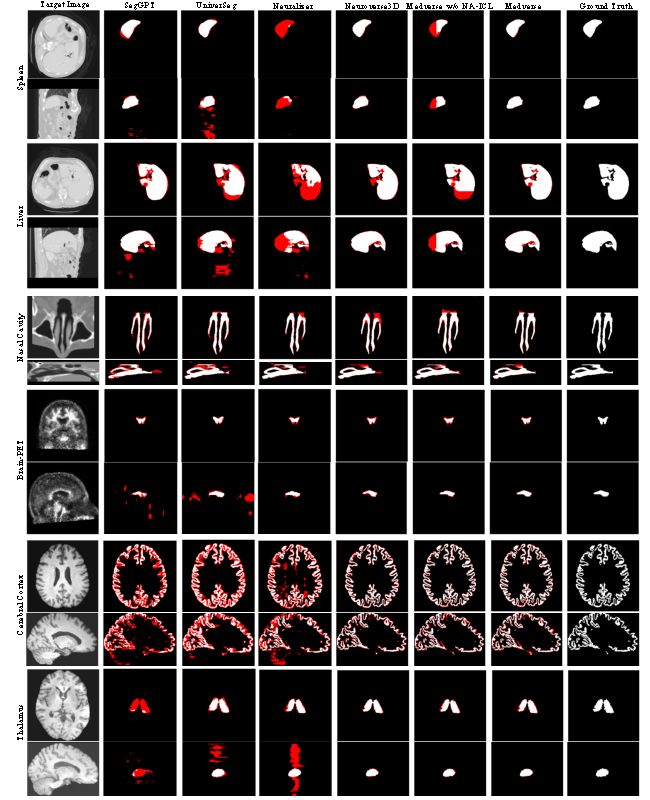
\includegraphics[width=0.92\textwidth]{sup_quantitative1.pdf}
\caption{Additional quantitative results for segmentation tasks.}
\label{fig:sub_quan1}
\end{figure*}

\begin{figure*}[htbp]
\centering
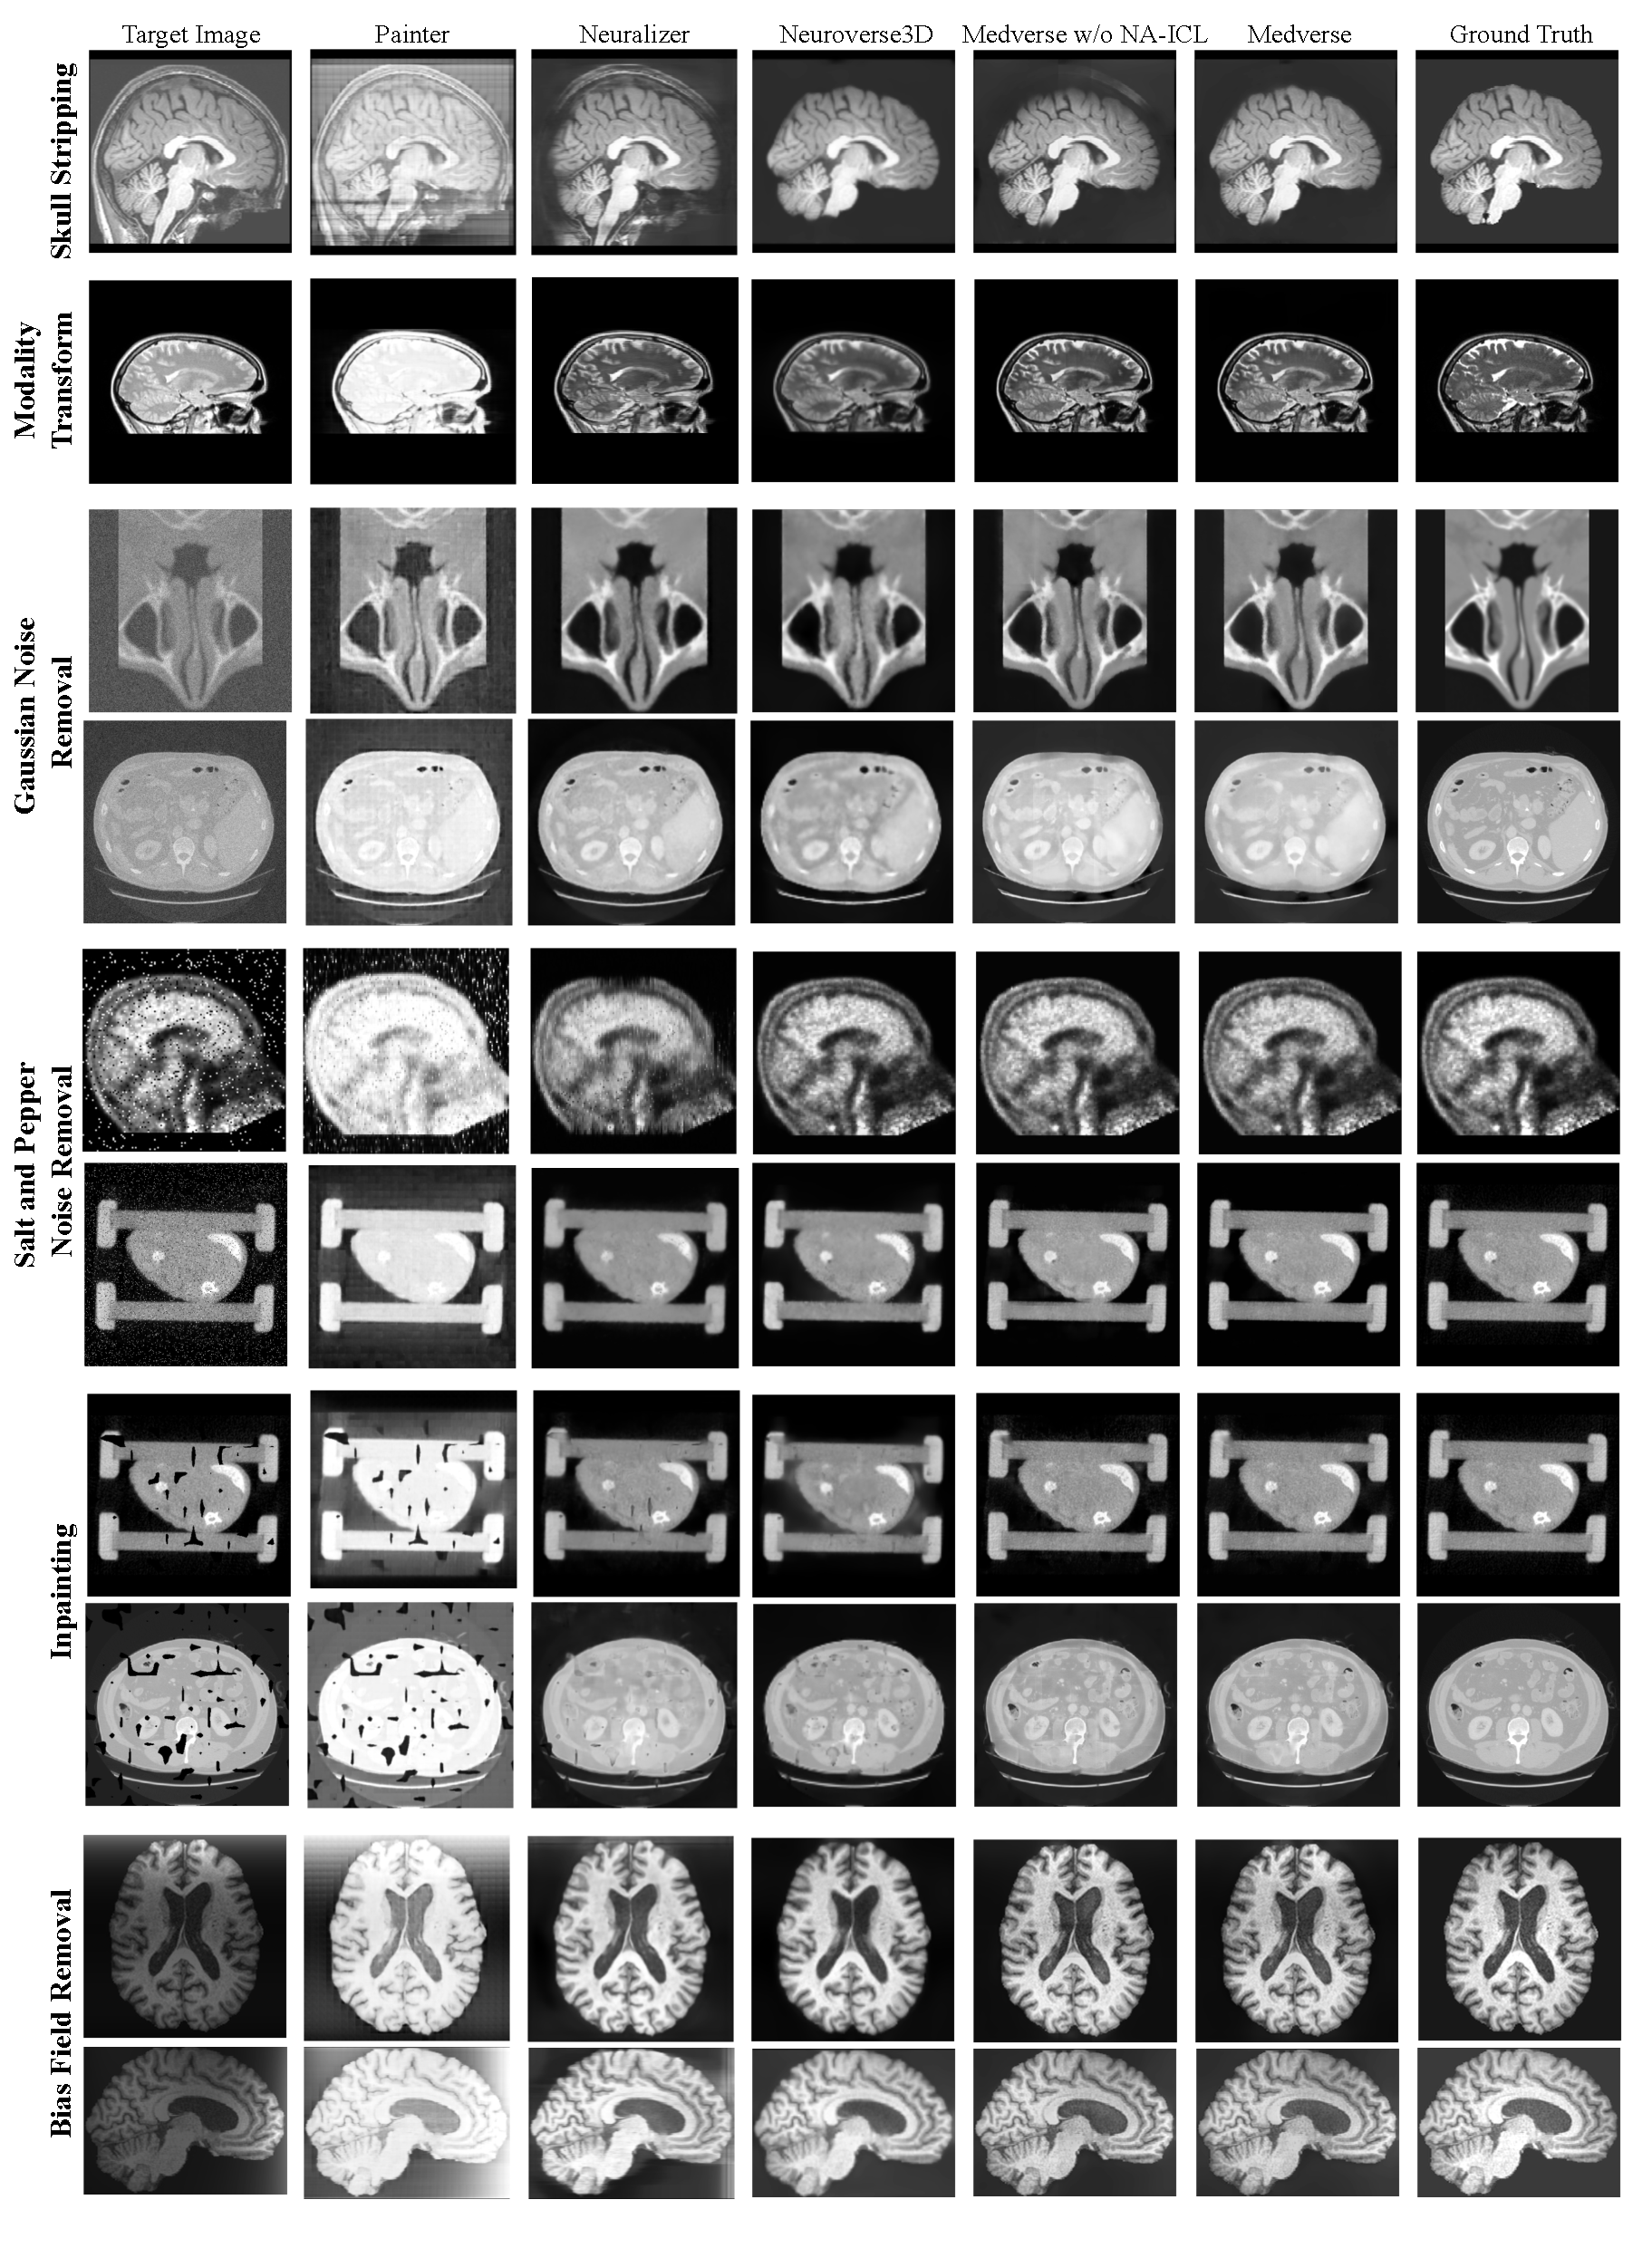
\includegraphics[width=0.90\textwidth]{sup_quantitative2.pdf}
\caption{Additional quantitative results for transformation and enhancement tasks.}
\label{fig:sub_quan2}
\end{figure*}


\vspace{0.4em}
\noindent\textbf{More Segmentation Results.} Table~\ref{tab:more_seg_comparison} presents the performance of various ICL models on the validation set. It can be observed that our model achieves competitive results on BraTs whole tumor segmentation and vascular segmentation, and significantly outperforms other models in terms of average performance.

\begin{table*}[htbp]
\centering
\setlength{\tabcolsep}{5pt}
\begin{tabular}{l l r r r r r}
\toprule
\textbf{Target} & \textbf{Organ \& Modality} & \textbf{UniverSeg} & \textbf{SegGPT} & \textbf{Neuralizer} & \textbf{Neuroverse3D} & \textbf{Medverse} \\
\midrule
BraTs Whole Tumor            & Brain MRI T1        & 18.13 & 18.39 &  7.32 & \textbf{81.85} & \underline{81.39} \\
BraTs Whole Tumor           & Brain MRI T2       & 34.63 & 30.77 &  6.12 & \underline{89.35} & \textbf{89.59} \\
Topcow                      & Brain MRA      & 38.70 & 24.69 & 13.07 & \textbf{82.30} & \underline{78.98} \\
Cerebral Cortex   & Brain MRI T1  & 69.82 & 50.05 & 66.91 & \underline{87.57} & \textbf{88.44} \\
Hippocampus              & Brain MRI T1  & 42.70 & 23.06 & 60.28 & \textbf{82.14} & \underline{81.42} \\
Thalamus           & Brain MRI T1  & 32.91 & 23.85 & 40.31 & \underline{86.23} & \textbf{86.80} \\
Lateral Ventricle & Brain MRI T1  & 57.90 & 46.13 & 60.02 & \underline{87.41} & \textbf{88.31} \\
Putamen            & Brain MRI T1  & 46.62 & 22.66 & 50.47 & \textbf{85.99} & \underline{85.35} \\
Amygdala           & Brain MRI T1  & 26.56 & 4.53 & 46.38 & \textbf{69.40} & \underline{63.74} \\
PROMISE12                   & Prostate MRI      & \underline{60.50} & 49.93 & 59.15 & 35.02 & \textbf{87.81} \\
MSD Heart                  & Cardiac CT        & \underline{75.18} & 43.94 & 65.12 & 70.30 & \textbf{82.81} \\
RAOS Liver             & Abdominal CT      & 55.81 & 48.54 & 54.54 & \underline{83.71} & \textbf{93.53} \\
RAOS Kidney            & Abdominal CT      & 37.93 & 38.89 & \underline{39.65} & 37.91 & \textbf{86.83} \\
RAOS Stomach           & Abdominal CT      & 25.91 & 22.72 & 16.83 & \underline{32.80} & \textbf{47.69} \\
AMOS22 liver           & Abdominal CT      & 64.94 & 53.33 & 55.71 & \underline{79.09} & \textbf{95.43} \\
AMOS22 Kidney          & Abdominal CT      & 31.92 & 27.89 & 26.23 & \underline{46.80} & \textbf{93.79} \\
AMOS22 Stomach         & Abdominal CT      & \underline{24.64} & 16.16 & 13.42 & 21.68 & \textbf{56.48} \\
\midrule
\multicolumn{2}{c}{\textbf{Average}}                  & 43.81 & 32.09 & 40.09 & 68.21 & \textbf{81.67} \\
\bottomrule
\end{tabular}
\caption{Comparison of segmentation performance on validation set (Dice, \%) across datasets and modalities.}
\label{tab:more_seg_comparison}
\end{table*}

\vspace{0.4em}
\noindent\textbf{Computational Efficiency Comparison.} Table~\ref{tab:model_time} compares the computational efficiency when processing a $128 \times 128 \times 128$ 3D image patch. Medverse exhibits a relatively small parameter size and achieves an inference time comparable to Neuroverse3D, while being significantly faster than other 2D methods. Notably, the inclusion of the autoregressive context introduces only an additional 0.19 seconds of processing time, indicating that the inclusion of the autoregressive context adds minimal computational overhead. For a fair comparison, all 3D methods are evaluated without using sliding-window inference.

\begin{table}[!htpb]
\centering
\setlength{\tabcolsep}{3pt} 
\resizebox{0.7\textwidth}{!}{
\begin{tabular}{lcccc}
\toprule
& Inference Time (s) & Context (pair) & Parameters (M) \\
\midrule
Medverse & 1.16 & 8 3D & 71.05 \\
Medverse w/o NA-ICL & 0.97 & 8 3D & 71.05 \\
Neuroverse3D~\cite{hu2025building} & 1.01 & 8 3D & 70.85 \\
Neuralizer~\cite{czolbe2023neuralizer} & 4.96 & 32 2D & 1.27 \\
UniverSeg~\cite{butoi2023universeg} & 8.36 & 64 2D & 1.18 \\
Painter~\cite{wang2023images} & 31.35 & 1 2D & 307.72 \\
SegGPT~\cite{wang2023seggpt} & 184.89 & 8 2D & 307.72 \\
\bottomrule
\end{tabular}}
\caption{Inference time for a single $128 \times 128 \times 128$ 3D image patch on a V100 GPU along with corresponding model configurations. For Medverse, this includes the processing of both semantic and autoregressive contexts, whereas Medverse w/o NA-ICL excludes the autoregressive context. For 2D comparison methods, we adopt the optimal context settings reported in their respective papers and process the 3D image by splitting it into 128 individual 2D slices.}
\label{tab:model_time}
\end{table}

% \begin{algorithm}[t]
% \caption{Autoregressive Inference Pipeline of Medverse}
% \KwIn{Target image $\bm{x}$ of size $(H,W,D)$, semantic context $S$, patch size $I$}
% \KwOut{Prediction $\hat{\bm{y}}$}

% $T \leftarrow \left\lceil\log_2(\max\{H,W,D\}/I)\right\rceil + 1$ \tcp*{# scales}
% $\mathcal{A}^{(0)} \leftarrow \varnothing$ \tcp*{empty AR context}
% \For{$t = 1$ \KwTo $T$}{
%     Downsample $\bm{x}$ and $S$ to $(H^{(t)},W^{(t)},D^{(t)})$ \;
%     \eIf{$t == 1$}{
%         $\hat{\bm{y}}^{(1)} \leftarrow F\bigl(\bm{x}^{(1)},\, S^{(1)},\, \mathcal{A}^{(0)}\bigr)$ \;
%     }{
%         \ForEach{patch index $i$}{
%             Extract patch $\bm{x}^{(t)}_i$ of size $I^3$ \;
%             Crop $S^{(t)}_i$ at same location \;
%             Upsample corresponding region from $\mathcal{A}^{(t-1)}$ to $\mathcal{A}^{(t-1)}_i$ \;
%             $\hat{\bm{y}}^{(t)}_i \leftarrow F\bigl(\bm{x}^{(t)}_i,\, S^{(t)}_i,\, \mathcal{A}^{(t-1)}_i\bigr)$ \;
%         }
%         Stitch $\{\hat{\bm{y}}^{(t)}_i\}$ with overlap-average to obtain $\hat{\bm{y}}^{(t)}$ \;
%     }
%     $\mathcal{A}^{(t)} \leftarrow (\bm{x}^{(t)},\, \hat{\bm{y}}^{(t)})$ \tcp*{update context}
% }
% \Return $\hat{\bm{y}}^{(T)}$
% \end{algorithm}
